\chapter{Jets} \label{ch:jets}

\section{The proton-proton collision environment}\label{sec:jet_collisions}

As discussed in~\ref{subsec:qcd_pdfs}, the goal of proton-proton collision experiments is to understand the interactions
between fundamental particles, but due to QCD confinement it is impossible to simply collide the individual partons of interest.
Instead, complicated bound states of quarks and gluons are collided,
with the goal of measuring the processes that occur when constituent partons collide with each other.
As a result, proton-proton collision events create a very messy environment from which the hard-scatter process
has to be deduced.

QCD confinement also has the consequence that the final state quarks and gluons created in LHC collisions
can never be directly detected.
Instead, collimated sprays of hadrons, called jets, must be measured in order to attempt to reconstruct the
hard scattering process that gave rise to them.

Figure~\ref{fig:jet_tth_diagram} illustrates a typical proton-proton collision event,
in which two gluons annihilate to generate a Higgs boson along with a top-antitop quark pair.
Even though this is not a dijet or multijet production event,
it is useful for understanding all the parts of a proton-proton collision that must be considered when calculating the
predicted rates of multijet production.

\begin{figure}[h!]
    \centering
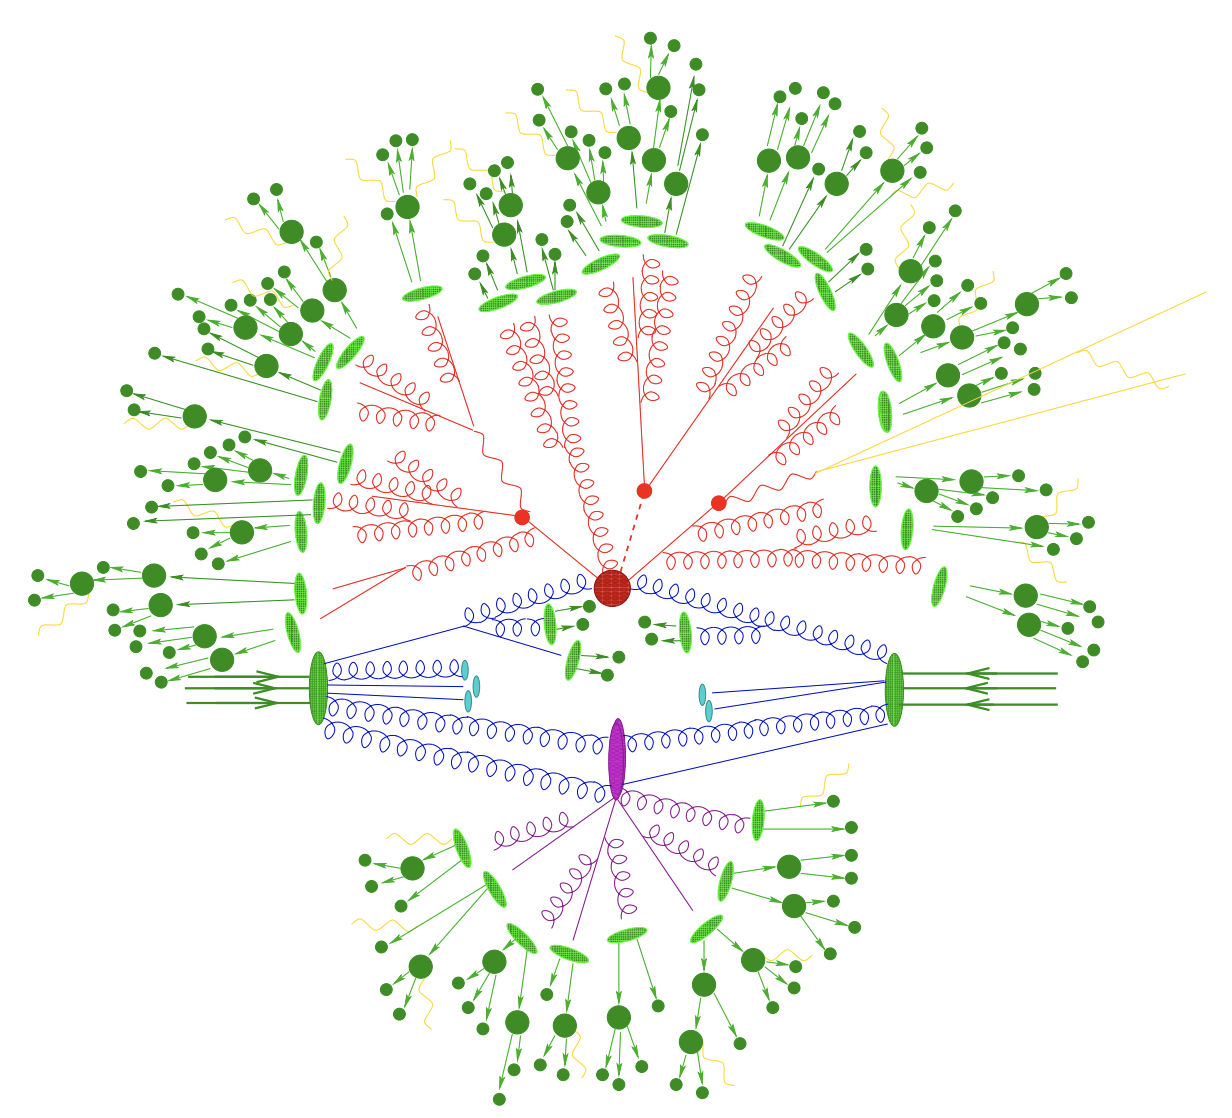
\includegraphics[width=0.6\linewidth]{jet_tth_diagram}
\caption{Diagram of a proton-proton collision event in which the hard scatter process is $t\bar{t}H$ production.
Illustrated are the initial state radiation, underlying event, hard-scatter process, final state parton shower,
fragmentation, hadron decays, and final state QED radiation.}
\label{fig:jet_tth_diagram}
\end{figure}\cite{sherpa-2004}

The incoming protons are illustrated by green blob with three incoming arrows to represent the constituent quarks.
The initial state parton showering, governed by QCD, is shown in blue.
The hard scatter process, in which two gluons annihilate to produce a Higgs boson and top-antitop pair is represented
by the large red circle.
Quarks and gluons from the incoming proton that do not participate in the hard scatter process can nonetheless interact
with each other, creating a so-called underlying event, shown in purple.
The Higgs decays to a quark-antiquark pair, shown in red, and all of the strongly-interacting final state quarks
and gluons undergo final state parton showering, also in red.
Once the final state parton shower particles reach a low enough energy, they hadronize, a non-perturbative process
indicated by the light green blobs.
The resulting hadrons then decay through various decay chains, shown in dark green.
Photon radiation, governed by QED, can occur at any of these stages, and is shown in yellow.

The final measured objects in the detector are the jets.
But every process leading up to the final state is quantum mechanical,
meaning that interference terms between the various processes lead to a fundamental and unresolvable ambiguity in the source of a given jet.

An event with 3 high-$pT$ jets could be explained by a $2\rightarrow3$ hard-scattering process,
or a $2\rightarrow2$ hard scattering process, with an additional jet arising from ISR or FSR, the underlying event,
or even from a hadronic decay.
All of these processes must be taken into account when calculating the rate of 3-jet events,
each contributing its own source of uncertainty.
The final rate calculation combines the perturbative QCD calculations for the matrix elements and parton showering
with empirically measured probability distributions for the non-perturbative parts of the collision,
including soft gluon emission, long-distance couplings, hadronization, and multi-parton interactions (MPI). 
As the number of jets in the final state increases, so does the complexity and uncertainty when calculating event rates.

Monte Carlo (MC) generators attempt to account for all of these effects to calculate the rate of multijet events at the LHC .
However, the MC estimates have very large uncertainties, for the reasons given above.
As a result, data driven estimation methods are used for determining the background rate of multijet events.

\section{Clustering Algorithms}\label{sec:jet_clustering}
\subsection{The $k_T$ algorithm}\label{subsec:jet_kt}
\subsection{The anti-$k_T$ algorithm}\label{subsec:jet_anti_kt}

\section{Substructure}\label{sec:jet_substructure}
\subsection{Boosted objects}\label{subsec:jet_boosted_substructure}
\subsection{Accidental substructure}\label{subsec:jet_accidental_substructure}

\section{Reconstruction in ATLAS}\label{sec:jet_reconstruction}
\subsection{Clustering}\label{subsec:jet_clustering}
\subsection{Calibration}\label{subsec:jet_calibration}
\subsection{Full and Fast Simulation Comparison}\label{subsec:jet_full_vs_fast_sim}
\subsection{Flavor Tagging}\label{subsec:jet_flavor_tagging}